\documentclass[10pt, oneside]{article} 
\usepackage{amsmath, amsthm, amssymb, calrsfs, wasysym, verbatim, bbm, color, graphics, geometry}
\usepackage[framemethod=TikZ]{mdframed}
\usepackage{xcolor}

\geometry{tmargin=.75in, bmargin=.75in, lmargin=.75in, rmargin = .75in}  

%%%% Styles %%%%

\newmdenv[
  skipabove=10pt,
  skipbelow=10pt,
  backgroundcolor=blue!3,
  linecolor=blue!60!black,
  linewidth=1pt,
  roundcorner=5pt,
]{thmbox}

\newmdenv[
  skipabove=10pt,
  skipbelow=10pt,
  backgroundcolor=gray!10,
  linecolor=gray!10!black,
  linewidth=1pt,
  roundcorner=5pt,
]{defbox}

\newmdenv[
  skipabove=10pt,
  skipbelow=10pt,
  backgroundcolor=yellow!5,
  linecolor=yellow!60!black,
  linewidth=0.8pt,
  roundcorner=5pt,
]{rembox}

% --- New versions
\newenvironment{theorembox}[1][]{\begin{thmbox}\begin{thm}[#1]}{\end{thm}\end{thmbox}}
\newenvironment{definitionbox}[1][]{\begin{defbox}\begin{defn}[#1]}{\end{defn}\end{defbox}}
\newenvironment{remarkbox}[1][]{\begin{rembox}\begin{rem}[#1]}{\end{rem}\end{rembox}}



\newcommand{\R}{\mathbb{R}}
\newcommand{\C}{\mathbb{C}}
\newcommand{\Z}{\mathbb{Z}}
\newcommand{\N}{\mathbb{N}}
\newcommand{\Q}{\mathbb{Q}}
\newcommand{\Cdot}{\boldsymbol{\cdot}}
\numberwithin{equation}{section}
\newtheorem{thm}{Theorem}[section]
\newtheorem{defn}{Definition}[section]
\newtheorem{conv}{Convention}
\newtheorem{rem}{Remark}
\newtheorem{lem}{Lemma}
\newtheorem{cor}{Corollary}
\newtheorem{proposition}{Proposition}[section]
\newtheorem{example}[thm]{Example}
\usepackage{enumitem}



\title{Real and Functional Analysis \\ \large Politecnico di Milano}
\author{Juan Pablo Vallejo Montañez}
\date{Academic Year 2025-2026}

\begin{document}

\maketitle
\tableofcontents

\vspace{.25in}

\textcolor{red}{OJO CON ESTO, EN TODAS LAS NOTAS HAY UN ERROR Y ES QUE LA DUPLA (X,A) ES MEASUTRABLE SPACE Y LA TRIPLETA (X,A,U) ES MEASURE SPACE REvisatr tpdo esto en todo el archivo que estoy seguro que la cague en mmas d eun sitio }

\section{Measurable Spaces}
\subsection{Measurable Sets and Spaces}
\begin{definitionbox}[\(\sigma \)-algrebra]
Let \(X\) be a set. A family of subsets \(\mathcal{A} \subseteq \mathcal{P}(X)\), is called a \(\sigma\)-algebra if it satisfies:

\begin{center}
\begin{minipage}{0.8\textwidth}
\begin{enumerate}[label=(\roman*)]
    \item \(\emptyset \in \mathcal{A}\) (\(\mathcal{A}\) is non-empty)  
    \item If \(E \in \mathcal{A} \Rightarrow \overline{E} \in \mathcal{A}\) (Closed under complement)
    \item Given a sequence of sets 
    \(\{E_n\}_{n\in \mathbb{N}} \subseteq \mathcal{A} \Rightarrow 
    \displaystyle \bigcup_{n=1}^{\infty} E_n \in \mathcal{A}\) 
    (Closed under countable union)
\end{enumerate}
\end{minipage}
\end{center}

where \(\mathcal{P}(X)\) denotes the power set of \(X\).\\
\\
(\(X,\mathcal{A})\) is \textbf{measurable space} when \(\mathcal{A}\) is a \textbf(\(\sigma\)-algebra). The elements of \(\mathcal{A}\) are called \textbf{measurable sets}
\end{definitionbox}

\textcolor{red}{Estas son las fomras que hay para determinar dos cosas que son bovias primero que el conjunyo X pertenence a la sigma algebra y que tambien es cerrado baajo intersecciones contables}\\
\textit{Notes:}
\begin{enumerate}[label=(\alph*)]
    \item From \textit{(i)} and \textit{(ii)}
    \begin{equation}S
         ( \emptyset^c = X)  \quad  \emptyset \in \mathcal{A} \Rightarrow X \in \mathcal{A}
    \end{equation}
    \item From the axioms, it follows that a \(\sigma\)-algebra is also closed under countable  intersections.
\begin{multline}
\forall n \in \mathbb{N} \quad E_n \in \mathcal{A}  \\ 
(X \setminus E_n) = \overline{E_n} \in \mathcal{A} \quad \textit{(ii)}
\\
\end{multline}
\begin{multline*}
\text{The sum of the complements of the elements of} \quad \mathcal{A} \quad  \text{belong to the set} \quad \mathcal{A}\\
\displaystyle \bigcup_{n \in \mathbb{N}} (X \setminus E_n) \in \mathcal{A} \quad \textit{(iii)}\\
\end{multline*}
Then this set and its completeme belong to \(\mathcal{A}\)
\begin{equation}
X \setminus [\displaystyle \bigcup_{n \in \mathbb{N}} X \setminus E_{n}] \in \mathcal{A}\\ 
\end{equation}
According to the De Morgan generalized form 
\begin{equation}
    \overline{\displaystyle \bigcup_{i \in I} A_{i}} \equiv \displaystyle \bigcap_{i \in I}\overline{A_i}
\end{equation}
\begin{equation}
    \overline{\displaystyle \bigcap_{i \in I} A_{i}} \equiv \displaystyle \bigcup_{i \in I}\overline{A_i}
\end{equation}
It follows that,
\begin{equation}
    \bigcup_{n \in \mathbb{N}} (X\setminus E_n) = \bigcup_{n \in \mathbb{N}} \overline E_n = \overline{\bigcap_{n \in \mathbb{N}}E_n} = X\setminus \bigcap_{n \in \mathbb{N}}E_n\\
\end{equation}
Taking (1.6) in (1.3)
\begin{equation}
    X \setminus (X \setminus \bigcap_{n \in \mathbb{N}} E_n ) = \bigcap_{n \in \mathbb{N}}E_n \in \mathcal{A}
\end{equation}
Finally a \(\sigma\)-algebra is closed under intersection
\end{enumerate}

\begin{thm}
    Let \(\mathcal{S} \subseteq \mathcal{P}(X)\), then there exists a \(\sigma\)-algebra \(\sigma (\mathcal{S})\) such that,
\begin{center}
\begin{minipage}{0.8\textwidth}
\begin{enumerate}[label=(\roman*)]
    \item \(\mathcal{S} \subseteq \sigma(\mathcal{S})\).  
    \item \(\forall \sigma\)-algebra \(\mathcal{A} \subseteq \mathcal{P(\text{X})}\) such that s \(\quad \mathcal{S} \subseteq \mathcal{A} \quad \text{such that} S \subseteq
    \mathcal{A} \quad \text{we have } \sigma_n (S) \subseteq \mathcal{A}\) 
\end{enumerate}
\end{minipage}
\end{center}
\end{thm}

\begin{definitionbox}[Borel Sets]
Let $(X, d)$ be a metric space, and let $\mathcal{G}$ denote the topology on $X$, i.e., the family of open subsets of $X$.
The $\sigma$-algebra generated by $\mathcal{G}$ is called the \textbf{Borel $\sigma$-algebra} denoted by $\mathcal{B(\mathbb{R})}$ .
The elements of this $\sigma$-algebra are called \textbf{Borel sets}.
\end{definitionbox}

\textcolor{yellow}{Read royden Cahpter 1 Page 18}

\begin{rem}
\textcolor{red}{Revisar esta definciion de topologia}

A topology $\mathcal{T}$ on a set $X$ can be defined as a collection of subsets of $X$ satisfying:
\begin{enumerate}
    \item $\emptyset, X \in \mathcal{T}$.
    \item For any collection $\{U_i\}_{i \in I}$, we have $\bigcup_{i \in I} U_i \in \mathcal{T}$ \quad (the union of any family of open sets is open).
    \item For any finite collection $\{U_i\}_{i=1}^{n}$, we have $\bigcap_{i=1}^{n} U_i \in \mathcal{T}$ \quad (the intersection of finitely many open sets is open).
\end{enumerate}
\end{rem}

\begin{defn}[$\sigma$-algebra generated by a set]
Let $S$ be a collection of subsets of $X$. The \textbf{$\sigma$-algebra generated by $S$}, denoted $\sigma(S)$, is the smallest $\sigma$-algebra that contains all elements of $S$.
\end{defn}

\textcolor{red}{REVISAR DEFINICION DE SIGMA ALGEBRA GENERADA y el ejemplo ademas de incluir el otro ejemplo de los borels sets}
\begin{example}
Let $X = \{1,2,3\}$. Then:
\[
P(X) = \{\emptyset, \{1\}, \{2\}, \{3\}, \{1,2\}, \{1,3\}, \{2,3\}, \{1,2,3\}\}.
\]
and let 
\[
S = \big\{ \{1,2\}, \{2,3\} \big\}.
\]

We can compute the $\sigma$-algebra generated by $S$ as follows:
\[
\sigma(S) = \{\emptyset, \{1,2\}, \{2,3\}, \{1,2,3\}, \{1,3\}\}.
\]

Indeed, $\sigma(S)$ is the intersection of all $\sigma$-algebras on $X$ that contain both $\{1,2\}$ and $\{2,3\}$:
\[
\sigma(S) = \bigcap_{\substack{\mathcal{A} \supset S \\ \mathcal{A}\text{ is a }\sigma\text{-algebra}}} \mathcal{A}.
\]
\end{example}

\begin{rem}
The collection of sets $\{\emptyset, X\}$ is the smallest possible $\sigma$-algebra on $X$.  
The collection $\mathcal{P}(X)$ (the power set of $X$) is the largest $\sigma$-algebra on $X$.
\end{rem}

\subsection{Measure}

\begin{definitionbox}[Measure]\label{def:measure}
Let $X$ be a general set and let $\mathcal{A}$ be a $\sigma$-algebra on $X$.
A function 
\[
\mu : \mathcal{A} \to \mathbb{R}_+ \cup \{+\infty\}
\]
is called a \textbf{measure} if:
\begin{enumerate}[label=(\roman*)]
    \item $\mu(\emptyset) = 0$,
    \item (\textbf{$\sigma$-additivity}) for every countable sequence $(E_k)_{k \in \mathbb{N}}$ of disjoint elements of $\mathcal{A}$,
    \[
    \mu\!\left( \bigcup_{k=1}^{\infty} E_k \right) = \sum_{k=1}^{\infty} \mu(E_k).
    \]
\end{enumerate}
\end{definitionbox}

\begin{rem}
Since we are dealing with a $\sigma$-algebra, a countable disjoint collection of Lebesgue-measurable sets is such that each pair of sets in the collection has empty intersection.\footnote{See \textit{Real Analysis}, Royden \& Fitzpatrick, 4th ed., Chapter 2, p. 30.}\\
Let $(E_k)_{k \in \mathbb{N}}$ be a countable collection of elements of $\mathcal{A}$.
For the sequence to be pairwise disjoint, we require:
\[
\forall\, k,j \in \mathbb{N},\ k \neq j \implies E_k \cap E_j = \emptyset.
\]
Hence, a sequence that contains $X$ cannot have any other element except the empty set.
Therefore, $\{\emptyset, X\}$ is a countable sequence of disjoint elements of $\mathcal{A}$.

\end{rem}

\begin{definitionbox}[Finite and $\sigma$-finite Measures]\label{def:finite}
A measure $\mu$ is said to be \textbf{finite} if $\mu(X) < \infty$.
On the other hand, $\mu$ is \textbf{$\sigma$-finite} if there exists a sequence $(E_k)_{k \in \mathbb{N}} \subseteq \mathcal{A}$ such that:
\[
X = \bigcup_{k=1}^{\infty} E_k, \quad \mu(E_k) < \infty \ \text{for all } k \in \mathbb{N}.
\]
\end{definitionbox}

\begin{definitionbox}[Measurable and Probability Spaces]\label{def:measurable}
Let $X$ be a set, $\mathcal{A}$ a $\sigma$-algebra on $X$, and $\mu$ a measure on $(X, \mathcal{A})$.
Then the triple $(X, \mathcal{A}, \mu)$ is called a \textbf{measurable space}.
In particular, if $\mu(X) = 1$, then $(X, \mathcal{A}, \mu)$ is called a \textbf{probability space}.
\end{definitionbox}

\textcolor{red}{Tengo dos ejemplos que faltan por añadir EL CARDINAL Y LA MEDIDA DE DIRAC junto con una imagen}
\\
\\
\\

\textcolor{red}{DEMOSTRAT TODAS ESTAS PROPIEDADES}
\begin{thm}[Properties of a Measure]\label{thm:measure-props}
Let $(X, \mathcal{A}, \mu)$ be a measure space. Then $\mu$ satisfies the following properties:
\begin{enumerate}[label=(\alph*)]
    \item \textbf{(\(\sigma\)-additivity) Finite additivity:}
    For every finite collection of pairwise disjoint measurable sets $(E_k)_{k \in \mathbb{N}} \subseteq \mathcal{A}$ with fixed $n \in \mathbb{N}$, then
    \[
    \mu\!\left( \bigcup_{k=1}^{n} E_k \right) = \sum_{k=1}^{n} \mu(E_k).
    \]
    \item \textbf{Monotonicity:}  
    If $A,B \in \mathcal{A}$ and $A \subseteq B$, then 
    \[
    \mu(A) \le \mu(B).
    \]

    \item \textbf{\(\sigma\)-subadditivity:}  
    For any countable collection of measurable sets $\{E_k\}_{k \in \mathbb{N}}$ (not necessarily disjoint), then
    \[
    \mu\!\left( \bigcup_{k=1}^{\infty} E_k \right) \le \sum_{k=1}^{\infty} \mu(E_k).
    \]

    \item \textbf{Continuity from below:}  
    For an increasing sequence $\{E_k\}_{k \in \mathbb{N}}$ in $\mathcal{A}$ with $E_k \uparrow E = \bigcup_{k=1}^{\infty} E_k$, we have
    \[
    \mu(E) = \lim_{k \to \infty} \mu(E_k).
    \]

    \item \textbf{Continuity from above:}  
    For a decreasing sequence $\{E_k\}_{k \in \mathbb{N}}$ in $\mathcal{A}$ with $E_k \downarrow E = \bigcap_{k=1}^{\infty} E_k$ and $\mu(E_1) < \infty$, we have
    \[
    \mu(E) = \lim_{k \to \infty} \mu(E_k).
    \]
\end{enumerate}
\end{thm}

\begin{definitionbox}[Set of Measure Zero]\label{def:measure-zero}
Given a general measurable space ($\mathcal{X},\mathcal{A},\mu$). A set $N \subseteq X$ is said to be a \textbf{null set} (or a set of measure zero) if
\[
\forall \varepsilon > 0,\ \exists \{A_k\}_{k \in \mathbb{N}} \subseteq \mathcal{A}
\ \text{such that}\ 
N \subseteq \bigcup_{k=1}^{\infty} A_k 
\quad \text{and} \quad 
\sum_{k=1}^{\infty} \mu(A_k) < \varepsilon.
\]
\end{definitionbox}

\textcolor{red}{TENER CUIDADO CON ESTA DEFINICION NO CREO QUE SEA UNA DEFINICON EEN SI SINO UNOA DEMOSTRACION O ALGO QUE SE DESGLOSA DE OTRA COSA}//
\textcolor{blue}{En si y de acuerdo a la clase un conjunto de medida cero es un conjunto que es medible y cuya metrica es 0 punto} //
\textcolor{green}{Revisar apuntes pagina 4, los conjuntos negligible tambien tienen medida cero pero no requiere que sean medibles, eso nos dice que el negiglgie es una propiedad geomtrica que se puede
inferir o determinaad¿dad sin la necesidad de una metrica por el contatrio, el conjunto de medida zero si se genera a partir de un medida}
\textcolor{red}{TRNGO UNA CONFUSION YA QUE LA METRICA SOLO SE DEFINE DESDE EL DOMINIO DE LA SIGMA ALGEBRA POR ENDE
NO TIENE SENTIDO DEFINIR LA MEDIDA PARA UN CONJUNTO QUE NO pertenence A LA SIGMA ALBREGRA ENTONCES COMO DIFERENCIO LOS CONJUNTOS negligible CON LOS DE ,EDIDA ZERO}
\begin{definitionbox}
    \[\mathcal{N}_\mu : \text{is the collection of sets of zero measure}
    \]
    \[\mathcal{T}_\mu : \text{is the collection of negligible sets}
    \]
\end{definitionbox}

\begin{example}\label{example:zero-measure}
Let \( X = \{a, b, c\} \) and define the family $\mathcal{A} = \{\emptyset, \{a\}, \{b,c\}, X\}$, which is also
the $\sigma$-algebra generated by $\{a\}$ ($\sigma_{a}$). 
Then \(\mathcal{A}\) is a \(\sigma\)-algebra on \(X\).

Define a measure \(\mu : \mathcal{A} \to [0, \infty]\) by:

\[
\mu(A) =
\begin{cases}
\mu(X) = \mu(\{a\}) := 1,\\[4pt]
\mu(\emptyset) = \mu(\{b,c\}) := 0.
\end{cases}
\]

Clearly, \(\mu\) is a measure on \((X, \mathcal{A})\).\\

Let
\[
N = \{b, c\} \in \mathcal{A} \; (\text{Is a measurable set}) \; \text{and} \; \mu(N)=0 \; \text{then} \; N \in \mathcal{N}_{\mu},
\]
where \(\mathcal{N}_{\mu}\) denotes the family of all \(\mu\)-null sets. \\

We have
\[
\{b\} \subset N, \quad \{c\} \subset N,
\]
\indent By monotonicity of the measure, 
\[
 \; \{b\} \subseteq N \Rightarrow \mu(\{b\}) \leq \mu(N) = 0 \; \text{then}\;\mu(\{b\})=0  
\]
\[
\text{but} \; \{b\}, \{c\} \notin \mathcal{A}, \quad \text{thus } \{b\}, \{c\} \in \mathcal{T}_\mu \setminus \mathcal{N}_\mu.
\]

Hence, \(\{b\} \; \text{and} \; \{c\} \) are negligible set but are not set of zero measure.

\end{example}
\textcolor{red}{SE PUEDE DEFINIR LA METRICA EN {b} SABOENDOPO QUE B NO HACE PARTE DE LA SIGMA LAGEBRA DEL ESPACIO ??? }


\begin{definitionbox}[Complete Measure Space]\label{def:complete-measurable-space}
A measure space \((X, \mathcal{A}, \mu)\) is said to be \textbf{complete} if
\[
\mathcal{T}_{\mu} \subseteq \mathcal{A}.
\]
In such a case, \(\mu\) is a \textbf{complete measure}, and \(\mathcal{A}\) is a \textbf{complete \(\sigma\)-algebra}.
\end{definitionbox}

\textcolor{red}{qUE UN ESPACIO SEA COMPLETO O NO DEPDENDE LA DE SIGMA ALGEBRA Y DE LA MEDIDA. lA SIGMA ALGEBRA ME DEIFNE QUE CONJUNTOS PUEDO MEDIR
POR ENDE QUE CONJUNTOS SON MEDIBLES O NO DEPDENDE DE LA SIGMA ALGEBRA. ADEMAS DE ESO, LA MEDIDA TAMBIEN ENTRA ANJUGAR ACA PORQUE ES ELLA LA QUE ME DICE 
QUE CONJUNTOS TIENEN MEDIDA 0( SOBRE ESOS SON LOS QUE YO EVALUO SI EL ESPACIO ES COMPLETO O NO)SI TENGO UN CONJUNTO CON MEDIDA DISTINTA DE CERO PERO CON 
SUBCONJUNTOS QUE NO PERTENCEN A LA SIGMA LAGEBRA NO HABRIA NINGUN TIPO DE PRONLEMA}

\begin{remarkbox}

According to the definition \ref{def:complete-measurable-space}, $\mathcal{T}_\mu$ and $\mathcal{N}_\mu$ must coincide. 
Consequently, there are no negligible sets that fail to be measurable. 
In this situation, $\mu$ is a complete measure, and $\mathcal{A }$ constitutes a complete $\sigma$-algebra.

\[
\mathcal{N}_{\mu} = \mathcal{T}_{\mu}
\quad \Longleftrightarrow \quad
(X, \mathcal{A}, \mu) \text{ is complete.}
\]

$\mathcal{A}$ contains all subsets of sets of measure zero, that is, if $E$ belongs to $\mathcal{A}$ and $\mu(E)=0$, then every subset of $E$ also 
belongs to $\mathcal{A}$ \\
If the measurable space is not complete, it is not guaranteed that the subsets of the sets in $\mathcal{A}$ are measurable.

\end{remarkbox}

\begin{example}
    From Example \ref{example:zero-measure}, this measurable space is not complete.
\end{example}

\begin{definitionbox}[True Almost Everywhere]
Consider a measurable space ($\mathcal{X},\mathcal{A},\mu$). A property \(P\) on \(X\) is said to be \textbf{true almost everywhere} if
\[
\{x \in X : P(x) \text{ is false}\} \in \mathcal{N}_{\mu}.
\]
If \((X, \mathcal{A}, \mu)\) is a measurable space, a property \(P\) is said to \textbf{hold almost everywhere} in \(X\)  
if there exists a measurable set \(N \in \mathcal{A}\) such that \(\mu(N) = 0\) and every \(x \in X \setminus N\) satisfies \(P\).  

\textit{In short, the set of elements that do not satisfy the property must be of measure zero.}



\end{definitionbox}
\begin{example}
\begin{enumerate}[label=(\roman*)]
    \item Let \( f, g : X \to \overline{\mathbb{R}} \).  
    We say that \( f \) and \( g \) are \textbf{equal almost everywhere} (a.e.) if
    \[
    \{x \in X : f(x) \ne g(x)\} \in \mathcal{N}_{\mu}.
    \]

    \item A function \( f : X \to \overline{\mathbb{R}} = [-\infty, +\infty] \) is said to be \textbf{finite almost everywhere} if
    \[
    \{x \in X : f(x) = \pm \infty\} \in \mathcal{N}_{\mu}.
    \]

    \item A function \( f : D_f \to \mathbb{R} \) is said to be \textbf{defined almost everywhere in \( X \)} if
    \[
    X \setminus D_f \in \mathcal{N}_{\mu}.
    \]
\end{enumerate}
\end{example}

\textcolor{red}{DO THE PROBE}
\begin{theorembox}[Equivalence Relation]
The relation of equality almost everywhere (a.e.) is an \textbf{equivalence relation}  
on the set of functions \( f : X \to \overline{\mathbb{R}} \).
\end{theorembox}

\begin{definitionbox}[Completion of a Measure Space]
Let \((X, \mathcal{A}, \mu)\) be a measure space.  
Define a new collection as
\[
\overline{\mathcal{A}}
:= 
\{\, E \subseteq X \mid \exists\, F, G \in \mathcal{A},\ F \subseteq E \subseteq G,\ 
\mu(G \setminus F) = 0 \,\}.
\]
Then \(\overline{\mathcal{A}}\) is a $\sigma$-algebra containing $\mathcal{A}$.

Define
\[
\overline{\mu} : \overline{\mathcal{A}} \longrightarrow \mathbb{R}_+,
\qquad
\overline{\mu}(E) := \mu(F),
\]
where \(F \in \mathcal{A}\) satisfies \(F \subseteq E \subseteq G\) with \(\mu(G \setminus F) = 0\).\\
Finally, $\overline{\mathcal{A}}$ is the \textbf{completed $\sigma$-algebra} and $\overline{\mu}$ is the \textbf{completed measure}.
\end{definitionbox}
\begin{remarkbox}[Intuitive Idea of Completion]
A non-complete measure space has “gaps”: some subsets of null sets are not measurable,
because the $\sigma$-algebra is too small to include them.
Completing the space means enlarging the $\sigma$-algebra by adding all subsets of null sets,
and extending the measure so that these new sets have measure zero.

In other words, completeness ensures that anything contained in a set of measure zero
is also measurable and of measure zero — filling the “holes” left by the original $\sigma$-algebra.\\

The condition $A \subseteq E \subseteq B$ with $\mu(B\setminus A)=0$ means that
$E$ is “trapped” between two measurable sets $A$ and $B$ that differ only on a
$\mu$-null set. In other words, $E$ coincides with $A$ up to a set of measure zero,
so $E$ can be obtained from $A$ by adding or removing negligible parts.

Hence, this formal definition expresses the idea that the completion
includes all sets that differ from measurable ones only by null parts.\\
\\
The completion of a measure space \((X, \mathcal{A}, \mu)\) can be equivalently defined as
\[
\overline{\mathcal{A}}
=
\{\, E \cup F \mid 
E \in \mathcal{A},\ 
F \subseteq N,\ 
N \in \mathcal{A},\ 
\mu(N) = 0
\,\}.
\]
Indeed, this is equivalent to the previous definition
\[
\overline{\mathcal{A}}
=
\{\, E \subseteq X \mid \exists\, A,B \in \mathcal{A},\ A \subseteq E \subseteq B,\ \mu(B \setminus A) = 0\,\}.
\]



The definition
\[
\overline{\mathcal{A}}
=
\{\,E \cup F \mid
E \in \mathcal{A},\ 
F \subseteq N,\ 
N \in \mathcal{A},\ 
\mu(N)=0\,\}
\]
formally expresses the idea of “filling the gaps” in the original $\sigma$-algebra.
Each new set is obtained by taking a measurable set $E$ and adding to it a subset $F$
of a $\mu$-null set $N$. 

Hence, the completion simply adds all subsets of null sets,
making the measure space complete without changing the values of the measure.

\begin{center}
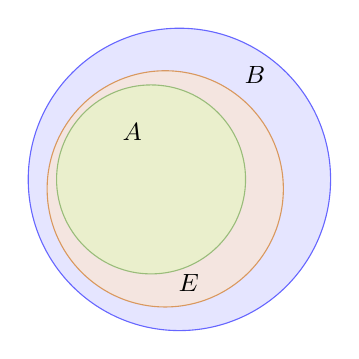
\begin{tikzpicture}[scale=1.2]
    % Conjuntos y etiquetas
    \draw[fill=blue!10, draw=blue!60] (0,0) circle (1.6cm); % B
    \draw[fill=green!20, draw=green!50!black] (-0.3,0) circle (1.0cm); % A
    \draw[fill=orange!20, draw=orange!80!black, opacity=0.6] (-0.15,-0.1) circle (1.25cm); % E aprox

    % Etiquetas
    \node at (-0.5,0.5) {\small $A$};
    \node at (0.8,1.1) {\small $B$};
    \node at (0.1,-1.1) {\small $E$};


\end{tikzpicture}
\end{center}

\textit{
The figure illustrates the definition of the completion of a measure space.
The set $E$ lies between two measurable sets $A$ and $B$ such that 
$\mu(B \setminus A) = 0$. 
The gray shaded region represents the \textbf{null part} where the two sets 
$A$ and $B$ may differ. 
Hence, $E$ can include or exclude any portion of this null part without 
changing its measure, which reflects the idea that in a complete measure space,any subset of a null set is also measurable and of measure zero.}








\end{remarkbox}



\begin{theorembox}[Completion Theorem]
Let \((X, \mathcal{A}, \mu)\) be a measure space.  
Then:
\begin{enumerate}[label=(\roman*)]
    \item \(\overline{\mathcal{A}}\) is a $\sigma$-algebra and \(\overline{\mathcal{A}} \supseteq \mathcal{A}\);
    \item \(\overline{\mu}\) is a \textbf{complete measure};
    \item The restriction of \(\overline{\mu}\) to \(\mathcal{A}\) coincides with \(\mu\), i.e.
    \[
    \overline{\mu}\big|_{\mathcal{A}} = \mu.
    \]
\end{enumerate}
\((X,\overline{\mathcal{A}},\overline{\mu})\) is a  \textbf{complete measure space}.\\
More precisely, it is the minimal complete measure space containing \((X,\mathcal{A},\mu)\), meaning that no smaller $\sigma$-algrebra can make the space complete. 
\end{theorembox}

\textcolor{red}{IF WE APPLY THE THEOREM TO A BOREL SIGMA ALGEBRA WE WILL HAVE THE LEBESGUE ONE, THE LEBESGUE SIGMA LAGEBRA IS AN EXTENSION OF THE BOREL ONE }


\begin{definitionbox}[Outer Measure]
Let \( X \) be a set.

A function 
\[
\mu^* : \mathcal{P}(X) \longrightarrow \overline{\mathbb{R}}_{+}
\]
is said to be an \emph{outer measure} on \( X \) if:
\begin{enumerate}[label=(\roman*)]
    \item \(\mu^*(\varnothing) = 0,\)
    \item if \(E_1 \subseteq E_2,\) then \(\mu^*(E_1) \leq \mu^*(E_2).\)
    \item (\(\sigma\)-subadditivity)
    \[
    \mu^*\!\left(\bigcup_{n=1}^{\infty} E_n\right)
    \leq 
    \sum_{n=1}^{\infty} \mu^*(E_n),
    \quad \forall\, \{E_n\}_{n\in\mathbb{N}} \subset \mathcal{P}(X).
    \]

\end{enumerate}
\end{definitionbox}

\textcolor{red}{IS COMPLICATED TO CREATE A MEASURE BY INSPECTION. THIS IS THE OBJECTIVE OF THE OOUTER MEASURE.
IT SO COMPLICATED FIND A MEASURE, CAN I APPROXIMATE A MESAURE, CAN I GET OSOMEETHING SIMILAR TO A MEASURE AND FROM THIS OBJECT GET FINALLY A MESAURE, THIS IS THE OBJECTIVE OF THE OUTER MEASURE.}
\textcolor{red}{HERE ALREADY IS MORE EASY THAN THE MEASURE BEACUSE WHEN DONT STAR FROM A SIGMA LAGEBRA, WE START FROM THE POWER SET THAT IS THE TRIVIAL SGIMA ALGEBRA OF A SET}

\begin{proposition}
Let $k \subseteq \mathcal{P}(x)$ and assume that $\varnothing \subseteq k$. $k$  is the 
For any set \(E \subseteq \mathbb{R}^n\), the \textbf{Lebesgue outer measure} is defined by
\[
m^*(E) = \inf\!\left\{ 
    \sum_{k=1}^{\infty} |I_k| 
    \; \middle| \; 
    E \subseteq \bigcup_{k=1}^{\infty} I_k, 
    \; I_k \text{ are closed cubes in } \mathbb{R}^n
\right\},
\]
where \(|I_k|\) denotes the volume (Lebesgue measure) of the cube \(I_k\).
\end{proposition}

\begin{remarkbox}[Intuitive Idea]
The Lebesgue outer measure approximates any set \(E \subseteq \mathbb{R}^n\)
by covering it with a countable collection of rectangles (or cubes) \(I_k\),
and summing up their total volumes. 
The infimum of all such sums gives the “best possible” approximation of the size of \(E\).
\end{remarkbox}

\begin{center}
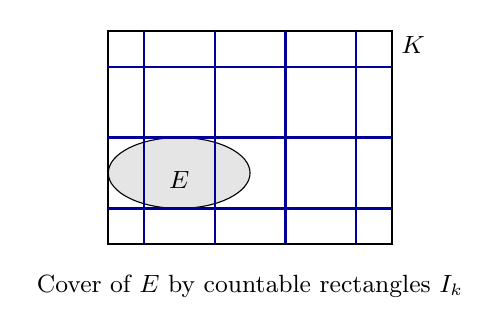
\begin{tikzpicture}[scale=0.9]
    \draw[thick] (-0.5,-0.5) rectangle (3.5,2.5);
    \node at (3.8,2.3) {\small $K$};
    \filldraw[fill=gray!20,draw=black] (0.5,0.5) ellipse (1cm and 0.5cm);
    \node at (0.5,0.4) {\small $E$};
    \draw[thick, blue!60!black] (-0.5,-0.5) grid[xstep=1,ystep=1] (3.5,2.5);
    \node[below] at (1.5,-0.8) {\small Cover of $E$ by countable rectangles $I_k$};
\end{tikzpicture}
\end{center}

\begin{remarkbox}[Notes]
This construction generalizes the intuitive idea of measuring a set 
by covering it with small rectangles (or intervals in $\mathbb{R}$). 
For a finite union of disjoint intervals, the outer measure coincides 
with the usual length (or volume).
\end{remarkbox}


\textcolor{red}{CARACTGEDORY CONDITION}
\textcolor{blue}{Tje caratheodry condition is like applying the additivity porpettyu of the measure
to the outer measure ans seeing which sets stisfyes it }




















\end{document}
